\documentclass{article}
\usepackage[a4paper,margin=4.72cm]{geometry}
\usepackage[utf8]{inputenc}
\usepackage[T1]{fontenc}

\usepackage[italian]{babel}
\usepackage{csquotes}

\usepackage{amsmath}
\usepackage{amssymb}
\usepackage{xurl}
\usepackage{hyperref}
\usepackage{listings}
\usepackage{graphicx}
\usepackage{xcolor}
\usepackage{bm}
\usepackage{listings}
\usepackage{float}

\usepackage[backend=biber,style=numeric,sorting=none]{biblatex}
\addbibresource{bibliografia.bib}

\AtBeginBibliography{%
  \small
  \setlength{\emergencystretch}{3em}%
}

\newcommand{\supcite}[2][]{\textsuperscript{\cite[#1]{#2}}}

\definecolor{Blue}{rgb}{0.2,0.2,0.9}
\definecolor{Green}{rgb}{0,0.6,0}
\definecolor{Gray}{rgb}{0.5,0.5,0.5}
\definecolor{Purple}{rgb}{0.58,0,0.82}
\definecolor{background}{rgb}{0.98,0.98,0.95}

\numberwithin{equation}{section}

\lstdefinestyle{mystyle}{
    backgroundcolor=\color{background},   
    commentstyle=\color{Green},
    keywordstyle=\color{Blue},
    numberstyle=\tiny\color{Gray},
    stringstyle=\color{Purple},
    basicstyle=\ttfamily\footnotesize,
    breakatwhitespace=false,         
    breaklines=true,                 
    captionpos=b,                    
    keepspaces=true,                 
    numbers=left,                    
    numbersep=5pt,                  
    showspaces=false,                
    showstringspaces=false,
    showtabs=false,                  
    tabsize=2
}
\lstset{style=mystyle}

\title{Progetto per il corso di \\ algoritmi numerici per la Fisica \\ \textbf{Equazione di Lane-Emden}}
\author{Manuel Gabriele Moretti}
\date{Settembre 2026}

\begin{document}
\maketitle

\begin{abstract}
    In questo progetto si è studiata numericamente l'equazione di Lane-Emden in funzione dell'indice politropico $n$ mediante il metodo RK4. In particolare, si è risolta per $n = \{0,1,3/2,2,3,4,5\}$, confrontando ove possibile la soluzione numerica con quella analitica. Per il caso $n = 3$ si è studiato il limite di Chandrasekhar, stimando la massa di Chandrasekhar e verificandone l'indipendenza dalla densità centrale della stella. Si è anche verificata la convergenza di RK4 stimando l'ordine di convergenza.
\end{abstract}

\section{Introduzione}
L'equazione di Lane-Emden è una forma adimensionale dell'equa-zione di Poisson per il potenziale gravitazionale di un fluido newtoniano, politropico e autogravitante a simmetria sferica. L'equazione\supcite[pagg.~86--88]{chandrasekhar1957} è 
\begin{equation}
\label{eq: equazione di Lane-Emden}
    \frac{1}{\xi^2}\frac{d}{d\xi}\bigg(\xi^2\frac{d\theta}{d\xi}\bigg) = -\theta(\xi)^n,
\end{equation}
dove $\xi$ è un raggio adimensionale e $\theta(\xi)$ è una funzione legata alla densità $\rho$ del gas tramite la relazione $\rho = \rho_c\theta(\xi)^n$ con $\rho_c$ la densità al suo centro. Il parametro $n$ ad esponente di $\theta$ è detto ``indice politropico''. In generale, un processo politropico è un processo termodinamico che obbedisce alla relazione
\begin{equation}
    pV^n = K,
\end{equation}
dove $p$ è la pressione, $V$ è il volume e $K$ è una costante, la quale descrive processi di espansione e compressione includendo il trasporto di calore. In questo caso, l'indice politropico appare nell'equazione di stato politropica assunta per questo sistema, data da
\begin{equation}
\label{eq: equazione di stato politropica}
    p = K\rho^{(n+1)/n}.
\end{equation}
Le condizioni iniziali assunte normalmente per l'equazione \eqref{eq: equazione di Lane-Emden} sono 
\begin{equation}
\label{eq: condizioni iniziali dell'equazione di Lane-Emden}
    \begin{cases}
        \theta(0) = 1, \\
        \theta'(0) = 0
    \end{cases},\quad \theta'(\xi) \equiv \frac{d\theta}{d\xi}.
\end{equation}
Le soluzioni dell'equazione di Lane-Emden quindi descrivono l'andamento della pressione e della densità in funzione del raggio $\xi$ e sono note come ``politropiche di indice $n$''. Se invece di un gas politropico si considerasse un gas isotermo, ovvero avente $n \to \infty$, pur sempre newtoniano autogravitante e a simmetria sferica, si otterrebbe l'equazione di Emden-Chandrasekhar. L'equazione\supcite[pagg.~155--157]{chandrasekhar1957} è
\begin{equation}
\label{eq: equazione di Emden-Chandraskhar}
    \frac{1}{\xi^2}\frac{d}{d\xi}\bigg(\xi^2\frac{d\psi}{d\xi}\bigg) = e^{-\psi},
\end{equation}
dove $\xi$ è un raggio adimensionale e $\psi$ è un parametro legato alla densità del gas tramite la relazione $\rho = \rho_ce^{-\psi}$ con $\rho_c$ la densità del gas nel suo centro. Le condizioni iniziali per l'equazione \eqref{eq: equazione di Emden-Chandraskhar} sono simili a quelle dell'equazione \eqref{eq: equazione di Lane-Emden}, ovviamente con la differenza che adesso si ha $\psi(0) = 0$ e non $\theta(0) = 1$.

\section{Equazione di Lane-Emden}
Per derivare l'equazione di Lane-Emden si assume prima di tutto che il fluido politropico sia in equilibrio idrostatico, ossia che valga la l'equazione 
\begin{equation}
\label{eq: equazione di equilibrio idrostatico}
    \frac{1}{\rho}\frac{dp}{dr} = -\frac{Gm(r)}{r^2},
\end{equation}
dove $m(r)$ è in generale funzione della distanza dal centro del sistema. Dato che la massa è conservata, vale l'equazione di continuità
\begin{equation}
\label{eq: equazione di continuità}
    \frac{dm}{dr} = 4\pi r^2\rho.
\end{equation}
Differenziando nuovamente rispetto ad $r$ l'equazione \eqref{eq: equazione di equilibrio idrostatico} si ottiene
\begin{equation}
    \frac{d}{dr}\bigg(\frac{dp}{dr}\bigg) = \frac{2Gm}{r^3} - \frac{G}{r^2}\frac{dm}{dr} = -\frac{2}{\rho r}\frac{dp}{dr} - 4\pi G\rho,
\end{equation}
dove nel secondo passaggio si è sostituita l'equazione \eqref{eq: equazione di continuità}. Moltiplicando ad ambo i membri per $r^2$ l'equazione appena ottenuta e raccogliendo i termini dipendenti da $dp/dr$ al membro di sinistra è possibile scrivere
\begin{equation}
    r^2\frac{d}{dr}\bigg(\frac{1}{\rho}\frac{dp}{dr}\bigg) + \frac{2r}{\rho}\frac{dp}{dr} = \frac{d}{dr}\bigg(\frac{r^2}{\rho}\frac{dp}{dr}\bigg) = -4\pi G\rho r^2.
\end{equation}
Dividendo adesso per $r^2$ e sostituendo l'equazione di stato politropica \eqref{eq: equazione di stato politropica} insieme alla relazione $\rho = \rho_c\theta(r)^n$ si ottiene
\begin{equation}
    \frac{1}{r^2}\frac{d}{dr}\bigg[r^2K\rho_c^{1/n}(n+1)\frac{d\theta}{dr}\bigg] = -4\pi G\rho_c \theta(r)^n.
\end{equation}
Definendo adesso il raggio $r$ tramite il parametro adimensionale $\xi$ come
\begin{equation}
    r = \alpha\xi,\quad \alpha^2 \equiv \frac{(n + 1)}{4\pi G}K\rho_c^{(1 - n)/n},
\end{equation} 
si ricava proprio l'equazione di Lane-Emden \eqref{eq: equazione di Lane-Emden}. Inoltre, dalla relazione \eqref{eq: equazione di stato politropica} è possibile trovare l'andamento della pressione, ossia
\begin{equation}
    p = K\rho_c^{(n+1)/n}\theta(\xi)^{n+1},
\end{equation}
mentre il profilo di temperatura può essere determinato ricordando che, se il gas è ideale, l'equazione di stato per la pressione è
\begin{equation}
    p = \frac{k_B\rho T}{\mu},
\end{equation}
per cui 
\begin{equation}
    T = \frac{K\mu}{k_B}\rho_c^{1/n}\theta(\xi),
\end{equation}
dove $\mu$ è la massa molecolare media.


\subsection{Soluzioni analitiche}
Come già anticipato, la soluzione dell'equazione di Lane-Emden consiste in una funzione $\theta(\xi)$. Tuttavia, tale soluzione dipende dal valore dell'indice politropico $n$, pertanto la soluzione dell'equazione \eqref{eq: equazione di Lane-Emden} si denota con $\theta_n(\xi)$. In generale, l'equazione di Lane-Emden deve essere risolta numericamente, ciò nonostante per certi valori di $n$ esistono delle soluzioni analitiche esatte che possono eventualmente usate per verificare i metodi di risoluzione numerici; tali valori sono $n = \{0,1,5\}$ e sono gli unici per la quale l'equazione di Lane-Emden è integrabile nei casi di sistemi a simmetria sferica. Per valori di $n \in [0,5)$ le soluzioni sono continue e finite, e il raggio $r$ della stella è dato da $r = \alpha\xi_s$ dove $\xi_s$ è il primo zero della soluzione, ovvero tale che $\theta_n(\xi_s) = 0$. Inoltre, conoscendo l'andamento della densità $\rho$ in funzione di $\theta(\xi)$, la massa $M$ della stella può essere determinata integrando il profilo di densità lungo il raggio tra $\xi = 0$ e $\xi = \xi_s$.

\paragraph{Soluzione per $\bm{n = 0}$.} Nel caso in cui $n = 0$, l'equazione \eqref{eq: equazione di Lane-Emden} si riduce a 
\begin{equation}
    \frac{1}{\xi^2}\frac{d}{d\xi}\bigg(\xi^2\frac{d\theta_0}{d\xi}\bigg) + 1 = 0.
\end{equation}
Quest'ultima può essere moltiplicata per $\xi^2$ in modo da poter integrare una prima volta su $d\xi$ la derivata totale nel membro di sinistra ottenendo
\begin{equation}
    \xi^2\frac{d\theta_0}{d\xi} = -\frac{\xi^3}{3} + K,
\end{equation}
la quale, se divisa ambo i membri per $\xi^2$, può essere integrata una seconda volta ottenendo così 
\begin{equation}
    \theta_0(\xi) = -\frac{\xi^2}{6} - \frac{K}{\xi} + K'.
\end{equation}
Imponendo ora le condizioni iniziali \eqref{eq: condizioni iniziali dell'equazione di Lane-Emden} si trova che le costanti di integrazioni sono rispettivamente $K = 0$ e $K' = 1$, pertanto 
\begin{equation}
\label{eq: soluzione per n = 0}
    \theta_0(\xi) = 1 - \frac{\xi^2}{6},
\end{equation}
la quale si annulla chiaramente per $\xi \equiv \xi_s = \sqrt{6}$.

\paragraph{Soluzione per $\bm{n = 1}$.} Nel caso in cui $n = 0$, l'equazione \eqref{eq: equazione di Lane-Emden} si riduce a 
\begin{equation}
    \frac{1}{\xi^2}\frac{d}{d\xi}\bigg(\xi^2\frac{d\theta_1}{d\xi}\bigg) + \theta_1(\xi) = 0.
\end{equation}
Per risolvere questa equazione si assume che la funzione $\theta_1(\xi)$ possa essere espressa come una serie di potenze 
\begin{equation}
\label{eq: ansatz soluzione per n = 1}
    \theta_1(\xi) = \sum_{k=0}^\infty a_k\xi^k,
\end{equation}
che se sostituita nell'equazione da risolvere porta a
\begin{equation}
    \sum_{k=0}^\infty k(k - 1)a_k\xi^{k - 2} + 2\sum_{n=0}^\infty ka_k\xi^{k - 2} + \sum_{k = 0}a_k\xi^k = 0.
\end{equation}
Adesso, dato che l'esponente di $\xi$ deve essere positivo si può far partire la somma dei primi due termini della precedente equazione da $k = 2$, invece per il terzo termine si può effettuare la sostituzione $k \mapsto g - 2$ e successivamente rinominare $g \mapsto k$; in questo modo si ottiene la relazione
\begin{equation}
    \sum_{k = 2}^\infty[k(k + 1)a_k + a_{k - 2}]\xi^{k - 2} = 0,
\end{equation}
la quale può annullarsi se e solo se il coefficiente della serie è nullo, portando alla seguente relazione di ricorsione per i coefficienti di espansione
\begin{equation}
    a_{k - 2} = -k(k + 1)a_k,
\end{equation}
che rinominando la variabile $k - 2$ si può riscrivere come
\begin{equation}
    a_{k + 2} = -\frac{a_k}{(n + 2)(n + 3)}.
\end{equation}
Applicando le condizioni iniziali \eqref{eq: condizioni iniziali dell'equazione di Lane-Emden} all'ansatz in equazione \eqref{eq: ansatz soluzione per n = 1} si trova che $\theta(0) = 1$ implica che $a_0 = 1$, ma allora $\theta'(0) = 0$ implica che $a_0 = 0$. Quindi, i coefficienti di espansione $a_k$ con indice $k$ dispari sono tutti nulli, mentre quelli con indice dispari sono legati dalla relazione di ricorsione, di conseguenza $\theta_1(\xi)$ risulta essere
\begin{equation}
    \theta_1(\xi) = 1 - \frac{\xi^2}{6} + \frac{\xi^4}{120} - \frac{\xi^6}{5040} + \cdots,
\end{equation}
che coincide con lo sviluppo in serie di Taylor di $\sin(\xi)/\xi$. Dunque, la soluzione dell'equazione di Lane-Emden per $n = 1$ è
\begin{equation}
\label{eq: soluzione per n = 1}
    \theta_1(\xi) = \frac{\sin(\xi)}{\xi},
\end{equation}
in accordo con le condizioni iniziali. Dalla forma di $\theta_1(\xi)$ segue immediatamente che questa si annulla per la prima volta per $\xi \equiv \xi_s = \pi$, e ovviamente per tutti i multipli interi di $\pi$. 

\paragraph{Soluzione per $\bm{n = 5}$.} Nel caso in cui $n = 5$ l'equazione \eqref{eq: equazione di Lane-Emden} diventa
\begin{equation}
    \frac{1}{\xi^2}\frac{d}{d\xi}\bigg(\xi^2\frac{d\theta_1}{d\xi}\bigg) + \theta_5(\xi)^5 = 0.
\end{equation}
Per risolvere questa equazione si può seguire lo stesso metodo usato per il caso $n = 1$ imponendo l'ansatz \eqref{eq: equazione di Lane-Emden}. Come in quel caso, i coefficienti con indice dispari sono tutti nulli e l'espressione della soluzione risulta essere
\begin{equation}
    \theta_5(\xi) = 1 - \frac{\xi^2}{6} + \frac{\xi^4}{24} - \frac{5}{432}\xi^6 + \cdots,
\end{equation}
la quale corrisponde all'espansione in serie di Taylor di $(1 + \xi^2/3)^{-1/2}$. Dunque, la soluzione dell'equazione di Lane-Emden per $n=5$ è
\begin{equation}
\label{eq: soluzione analitica per n = 5}
    \theta_5(\xi) = \bigg(1 + \frac{\xi^2}{3}\bigg)^{-1/2}.
\end{equation}
Quando $n = 5$, la soluzione restituisce un valore finito per la massa della stella, ma questa risulta essere di raggio infinito, per cui la politropa completa non rappresenta una soluzione di significato fisico. 
\bigskip

Nelle applicazioni pratiche ricoprono un ruolo fondamentale le soluzioni analitiche esprimibili tramite l'espansione in serie di potenze convergenti, intorno ad un dato punto iniziale. Tipicamente, il punto di espansione corrisponde con il centro della stella a $\xi = 0$. Tuttavia, questo punto è un punto singolare dell'equazione \eqref{eq: equazione di Lane-Emden} su cui si devono definire oltretutto anche le condizioni iniziali di suddetta equazione. Si può dimostrare che l'equazione \eqref{eq: equazione di Lane-Emden} ha una soluzione in serie di potenze convergenti della forma 
\begin{equation}
    \theta_n(\xi) = \theta_n(0) - \frac{\theta_n(0)^n}{6}\xi^2 + \frac{n\theta_n(0)^{n - 1}}{120}\xi^4 + O(\xi^6).
\end{equation}
Imponendo quindi le condizioni iniziali \eqref{eq: condizioni iniziali dell'equazione di Lane-Emden} si ottiene
\begin{equation}
\label{eq: sviluppo intorno all'origine}
    \theta_n(\xi) = 1 - \frac{\xi^2}{6} + \frac{n}{120}\xi^4 + O(\xi^6).
\end{equation}
Questo sviluppo viene utilizzato per approssimare la soluzione nell'intervallo $0 \leq \xi \leq \varepsilon$, vicino al centro della stella. I valori della funzione e della sua derivata a $\xi = \varepsilon$ forniscono poi le condizioni iniziali per l'integrazione numerica dell'equazione completa. A tale scopo, l'equazione differenziale del secondo ordine viene riscritta come un sistema di due equazioni differenziali del primo ordine.

\section{Limite di Chandrasekhar}
La ``massa di Chandrasekhar'' è la massa al di sopra della quale la pressione di degenerazione del nucleo della stella diventa insufficiente a mantenere l'equilibrio e bilanciare il campo gravitazionale della stessa. Le stelle della sequenza normale comprimono gli atomi di idrogeno formando atomi di elio attraverso la fusione nucleare, generando enormi quantità di energia. Con il consumo dell'idrogeno, il nucleo delle stelle si comprime ulteriormente consentendo all'elio e ai nuclei più pesanti di fondersi, fino a generare nuclei di ferro, questi sono gli ultimi atomi che possono essere generati dalle stelle tramite fusione durante l'evoluzione stellare. Il passo successivo dipende dalla massa della stella: quelle aventi una massa al di sotto di un certo valore di soglia diventano nane bianche, mentre quelle al di sopra di tale soglia possono diventare stelle di neutroni o buchi neri. Il valore di soglia è detto ``limite di Chandrasekhar'' e la massa è la massa di Chandrasekhar, indicata nel seguito con $M_C$. 

Le nane bianche resistono il collasso gravitazionale principalmente attraverso la pressione di degenerazione elettronica, a differenza di quanto accade per le stelle appartenenti alla sequenza principale, che invece resistono al collasso tramite la pressione termica. Il limite di Chandrasekhar è la conseguenza della competizione tra la gravità e la pressione di degenerazione elettronica. Questa pressione è un effetto quantistico che deriva dal principio di esclusione di Pauli: poiché gli elettroni sono fermioni, due elettroni non possono trovarsi nello stesso stato, quindi riempiono progressivamente gli stati disponibili, a partire da quelli di energia più bassa fino a un livello massimo, detto energia di Fermi. Quando il gas di elettroni viene compresso, lo stesso numero di elettroni deve occupare un volume più piccolo. Di conseguenza, aumenta la densità elettronica e gli elettroni sono costretti a occupare stati con momento ed energia sempre maggiori. L'energia complessiva del gas aumenta quindi al diminuire del volume. Per comprimere ulteriormente il gas è necessario compiere lavoro contro questa crescita di energia: macroscopicamente, questa resistenza alla compressione si manifesta come pressione di degenerazione elettronica. Con una compressione sufficiente, gli elettroni vengono forzati nei nuclei tramite cattura elettronica, alleviando la pressione\supcite[cap.~X]{chandrasekhar1957}. 

Nel caso non relativistico, la pressione di degenerazione elettronica dà origine a un'equazione di stato della forma $p = K_1\rho^{5/3}$ portando quindi all'equazione di Lane-Emden con indice politropico $n = 3/2$. Tuttavia, all'aumentare della massa, la maggiore compressione costringe gli elettroni a occupare stati con quantità di moto ed energie sempre più elevate, fino a quando tali energie non sono più trascurabili rispetto alla loro energia di riposo: le velocità degli elettroni si avvicinano alla velocità della luce e si deve tenere conto degli effetti relativistici. Nel limite fortemente relativistico, l'equazione di stato assume la forma $p = K_2\rho^{4/3}$, portando all'equazione di Lane-Emden con indice $n = 3$ e ad un valore di massa totale della stella $M_C$ costante. Per un trattamento completamente relativistico, l'equazione di stato utilizzata interpola tra le equazioni $p = K_1\rho^{5/3}$ per valori piccoli di $\rho $ e $p = K_2\rho^{4/3}$ per valori grandi di $\rho $. In questo caso, il raggio del modello diminuisce ancora con la massa, ma diventa zero in corrispondenza di $M_C$\supcite[cap.~XI]{chandrasekhar1957}.

\subsection{Massa di Chandrasekhar}
L'equazione della nana bianca\supcite[pgg.~208-209]{chandrasekhar1935} è un'equazione differenziale della forma 
\begin{equation}
\label{eq: equazione della nana bianca}
    \frac{1}{\eta^2}\frac{d}{d\eta}\bigg(\eta^2\frac{d\phi}{d\eta}\bigg) + [\phi(\eta)^2 - C]^{3/2} = 0
\end{equation}
con condizioni iniziali 
\begin{equation}
    \begin{cases}
        \phi(0) = 1 \\
        \phi'(0) = 0
    \end{cases},
\end{equation}
dove $\eta$ è una distanza radiale adimensionale, $\phi(\eta)$ misura la densità della nana bianca e $C$ è una costante legata alla densità della stella nel suo centro. Il bordo dell'equazione $\eta = \eta_\infty$ è definito dalla condizione 
\begin{equation}
    \phi(\eta_\infty) = \sqrt{C},
\end{equation}
in modo che l'intervallo di valori di $\phi(\eta)$ sia dato da $\sqrt{C} \le \phi(\eta) \le 1$. Questa condizione al bordo equivale a richiedere che la densità si annulli per $\eta = \eta_\infty$.

Per derivare l'equazione \eqref{eq: equazione della nana bianca} si parte considerando la statistica di un gas di elettroni completamente degenere, ossia tale che gli stati quantici più bassi sono completamente occupati, dalla quale si ricava la pressione e la densità della nana bianca in termini del massimo momento $p_0$ acquistabile dall'elettrone definito da $x = p_0/m_ec$, con pressione e densità parametrizzate da $p = Af(x)$ e $\rho = Bx^3$ rispettivamente, dove
\begin{equation}
    A = \frac{\pi m_e^4c^5}{3h^3},\quad B = \frac{8\pi m_p\mu}{3}\bigg(\frac{m_ec}{h}\bigg)^3,
\end{equation}
\begin{equation}
    f(x) = x(2x^2 - 3)(x^2 + 1)^{1/2} + 3\sinh^{-1}{x}.
\end{equation}
Quando queste ultime espressioni sono sostituite nell'equazione di equilibrio idrostatico
\begin{equation}
     \frac{1}{r^2}\frac{d}{dr}\bigg(\frac{r^2}{\rho}\frac{dp}{dr}\bigg) = -4\pi G\rho
\end{equation}
si ottiene
\begin{equation}
    \frac{1}{r^2}\frac{d}{dr}\bigg[r^2\frac{d}{dr}\bigg(\sqrt{x^2 + 1}\bigg)\bigg] = -\frac{\pi GB^2}{2A}x^3.
\end{equation}
Denotando adesso la densità al centro della nana bianca come $\rho_0 = Bx_0^3$, cambiando variabile con $y^2 = x^2 + 1$ e definendo il raggio $r$ tramite il parametro adimensionale $\eta$ come
\begin{equation}
    r = \bigg(\frac{2A}{\pi GB^2}\bigg)^{1/2}\frac{\eta}{y_0},\quad y = y_0\phi(\eta),
\end{equation}
si ricava proprio l'equazione di Chandrasekhar per la nana bianca
\begin{equation}
    \frac{1}{\eta^2}\frac{d}{d\eta}\bigg(\eta^2\frac{d\phi}{d\eta}\bigg) + [\phi(\eta)^2 - C]^{3/2} = 0,\quad C = \frac{1}{y_0^2}.
\end{equation}
Quindi, il profilo di densità della stella è dato da 
\begin{equation}
    \rho(\eta) = By_0^3\bigg[\phi(\eta) - \frac{1}{y_0^2}\bigg]^{3/2} = 0,
\end{equation}
mentre la massa\supcite[pg.~211]{chandrasekhar1935} compresa in una sfera di raggio $\eta$ è calcolata tramite 
\begin{equation}
\label{eq; massa nana bianca generica}
    M(\eta) = -\frac{4\pi}{B^2}\bigg(\frac{2A}{\pi G}\bigg)^{3/2}\eta^2\frac{d\phi}{d\eta}.
\end{equation}
Ci sono due limiti dell'equazione \eqref{eq: equazione della nana bianca} particolarmente interessanti citati in precedenza. Il primo\supcite[pgg.~211--212]{chandrasekhar1935} consiste nel limite di bassa densità centrale: quando $\rho_0 \ll 1$, l'equazione della nana bianca si riduce all'equazione di Lane-Emden introducendo i parametri
\begin{equation}
    \xi = \sqrt{2}\eta,\quad \theta = \phi(\eta)^2 - 1 + x_0^2 + O(x_0^4),
\end{equation}
ottenendo al primo ordine 
\begin{equation}
    \frac{1}{\xi^2}\frac{d}{d\xi}\bigg(\xi^2\frac{d\theta}{d\xi}\bigg) = -\theta(\xi)^{3/2},
\end{equation}
soggetta alle condizioni iniziali
\begin{equation}
    \begin{cases}
        \theta(0) = x_0^2 \\
        \theta'(0) = 0
    \end{cases}.
\end{equation}
Si noti che anche se l'equazione precedente ha effettivamente la forma di quella di Lane-Emden con indice politropico $n = 3/2$, le condizioni iniziali sono diverse da quelle definite in \eqref{eq: condizioni iniziali dell'equazione di Lane-Emden}. 

Il secondo\supcite[pgg.~213--214]{chandrasekhar1935} invece consiste nel limite ad alta densità centrale: quando $\rho_0 \to \infty$, ossia quando $y_0 \to \infty$ o equivalentemente $C \to 0$, l'equazione \eqref{eq: equazione della nana bianca} si riduce a
\begin{equation}
    \frac{1}{\eta^2}\frac{d}{d\eta}\bigg(\eta^2\frac{d\phi}{d\eta}\bigg) = -\phi^3,
\end{equation}
soggetta alle condizioni iniziali \eqref{eq: condizioni iniziali dell'equazione di Lane-Emden}. In questo caso quindi l'equazione della nana bianca corrisponde proprio all'equazione di Lane-Emden con indice politropico $n = 3$. Si noti che in questo limite il raggio $r$ tende a zero, mentre la massa della nana bianca\supcite[pg.~213]{chandrasekhar1935} tende ad un limite finito
\begin{equation}
\label{eq: massa di Chandrasekhar}
    \begin{aligned}
        M_C &= -\frac{4\pi}{B^2}\bigg(\frac{2A}{\pi G}\bigg)^{3/2}\eta^2\frac{d\phi}{d\eta}\bigg|_{\eta = \eta_\infty} \\
        &= -4\pi\bigg(\frac{3h^3}{8\pi m_p\mu m_e^3 c^3}\bigg)^2\bigg(\frac{2}{\pi G}\frac{\pi m_e^4 c^5}{3h^3}\bigg)^{3/2}\eta^2\frac{d\phi}{d\eta}\bigg|_{\eta = \eta_\infty} \\
        &= \bigg(-\eta^2\frac{d\phi}{d\eta}\bigg|_{\eta = \eta_\infty}\bigg)\frac{\sqrt{3\pi}}{2}\bigg(\frac{\hbar c}{G}\bigg)^{3/2}\frac{1}{m_p^2\mu^2} \\
        &= \omega\frac{\sqrt{3\pi}}{2}\bigg(\frac{\hbar c}{G}\bigg)^{3/2}\frac{1}{m_p^2\mu^2},
    \end{aligned}
\end{equation}
nota come la massa di Chandrasekhar. Nell'espressione precedente, la quantità $\omega$ è una costante legata alla soluzione dell'equazione di Lane-Emden con $n = 3$, infatti la si è definita come
\begin{equation}
    \omega \equiv -\eta^2\frac{d\phi}{d\eta}\bigg|_{\eta = \eta_\infty},
\end{equation}
il cui valore\supcite[tab.~1]{chandrasekhar1935} è $\omega \simeq 2.0182$. La massa di Chandrasekhar\supcite[pg.~214]{chandrasekhar1935} può poi essere scritta in funzione della massa solare $M_\odot$ come
\begin{equation}
    M_C = \frac{5.75}{\mu^2}M_\odot.
\end{equation}
La massa molecolare media $\mu$ è un parametro che indica, in media, quante unità di massa atomica sono presenti nel plasma per ogni elettrone libero. Tipicamente, una nana bianca è composta principalmente da carbonio-12 e ossigeno-16, quindi per entrambi i componenti il numero di nucleoni è esattamente il doppio del numero di elettroni. Di conseguenza, per qualsiasi miscela di carbonio e ossigeno, in media ci saranno sempre due nucleoni per ogni elettrone, portando quindi all'approssimazione $\mu \simeq 2$\supcite[pg.6]{chavanis2007}\supcite[pg.6]{thomas2011}. In questo modo, la massa di Chandrasekhar in masse solari è 
\begin{equation}
\label{eq: massa di Chadrasekhar in masse solari}
    M_C \simeq 1.44 M_\odot.
\end{equation}

\section{Analisi numerica}
Tornando all'equazione di Lane-Emden, si è già detto come l'integrazione numerica sia l'unico modo per ottenere delle soluzioni per ogni valore dell'indice politropico. In questo progetto si è quindi utilizzato il metodo di integrazione di Runge-Kutta del quarto ordine (RK4) per ottenere l'andamento di $\theta$ in funzione del raggio adimensionale $\xi$ e un'interpolazione lineare per trovare gli zeri della funzione per i valori di $n = \{0,1,3/2,2,3,4\}$, mentre per $n = 5$, dato che la soluzione non presenta zeri, si è dovuto definire un limite massimo $\xi_{max}$ e fermare l'integrazione. Per i valori dove è prevista una soluzione analitica si è potuto confrontare quanto ottenuto numericamente con i risultati teorici. Inoltre, si è determinato per ogni indice il profilo di densità $\rho/\rho_c$ in funzione di $\xi$. Nel caso in cui $n = 3$ si è anche stimata la massa di Chandrasekhar e verificata numericamente l'indipendenza di tale valore dalla densità centrale della stella. Il codice è riportato in appendice \ref{app: appendice}. 

\subsection{Metodo di Runge-Kutta del quarto ordine}

Il metodo RK4 è un metodo numerico per la soluzione di problemi ai valori iniziali. Si consideri un sistema di equazioni differenziali ordinarie del primo ordine nella forma
\begin{equation}
\label{eq: problema di Cauchy}
    \begin{cases}
        \dfrac{d\bm{y}}{dx} = \bm{f}(x,\bm{y}) \\[2ex]
        \bm{y}(x_0) = \bm{y}_0
    \end{cases},
\end{equation}
dove $\bm{y}$ è il vettore delle funzioni incognite e $\bm{f}$ ne determina le derivate. Un'equazione differenziale di ordine superiore può essere ricondotta a questa forma introducendo come nuove variabili la funzione incognita e le sue derivate fino all'ordine immediatamente inferiore a quello dell'equazione. L'intervallo di integrazione è suddiviso in una griglia di punti $x_i = x_0 + ih$, dove $h > 0$ è il passo di integrazione. Si indica con $\bm{y}_i$ l'approssimazione numerica della soluzione esatta $\bm{y}(x_i)$. Integrando l'equazione differenziale tra due punti consecutivi si ottiene la relazione esatta\supcite[pg.~132]{hairer1993}
\begin{equation}
\label{eq: forma integrale problema di Cauchy}
    \bm{y}(x_{i+1}) = \bm{y}(x_i)
    + \int_{x_i}^{x_{i+1}}dx\, \bm{f}(x,\bm{y}(x)).
\end{equation}
La costruzione di un metodo numerico consiste quindi nell'approssimare l'incremento della soluzione nell'intervallo considerato, senza conoscere preventivamente il suo andamento esatto.

Il metodo RK4 utilizza quattro valutazioni della funzione $\bm{f}$, dette stadi, per stimare tale incremento. Tipicamente esse sono definite da
\begin{equation}
\label{eq: stadi RK4}
    \begin{cases}
        \bm{k}_1 = \bm{f}(x_i,\bm{y}_i) \\[2ex]
        \bm{k}_2 = \bm{f}\bigg(x_i+\dfrac{h}{2}, \bm{y}_i+\dfrac{h}{2}\bm{k}_1\bigg) \\[2ex]
        \bm{k}_3 = \bm{f}\bigg(x_i+\dfrac{h}{2}, \bm{y}_i+\dfrac{h}{2}\bm{k}_2\bigg) \\[2ex]
        \bm{k}_4 = \bm{f}(x_i+h, \bm{y}_i+h\bm{k}_3)
    \end{cases}.
\end{equation}
Il primo stadio rappresenta la pendenza nel punto iniziale. Il secondo ed il terzo valutano la pendenza nel punto medio dell'intervallo, utilizzando due successive stime della soluzione in tale punto. Il quarto stadio valuta infine la pendenza all'estremo destro, a partire dalla stima ottenuta con il terzo stadio. Questi valori vengono combinati secondo la formula\supcite[pgg.~710--711]{press1992}
\begin{equation}
\label{eq: aggiornamento RK4}
    \bm{y}_{i+1} = \bm{y}_i
    + \frac{h}{6}\left(\bm{k}_1+2\bm{k}_2
    +2\bm{k}_3+\bm{k}_4\right).
\end{equation}
Si ottiene così una media pesata delle pendenze, nella quale le due valutazioni nel punto medio hanno peso doppio rispetto a quelle agli estremi. Le quantità $\bm{k}_j$ sono approssimazioni della derivata, mentre il fattore $h$ nella \eqref{eq: aggiornamento RK4} le converte in un incremento della soluzione. Il metodo è esplicito, poiché ogni stadio dipende soltanto da quantità già calcolate, ed è a un passo, poiché per determinare $\bm{y}_{i+1}$ è sufficiente conoscere $\bm{y}_i$, senza utilizzare i valori dei passi precedenti. Ogni avanzamento richiede quattro valutazioni di $\bm{f}$, ma non richiede il calcolo esplicito delle sue derivate.

L'ordine del metodo si determina confrontando un singolo passo numerico con lo sviluppo di Taylor della soluzione esatta. Supponendo che la soluzione sia sufficientemente regolare, tale sviluppo è
\begin{equation}
\label{eq: Taylor soluzione esatta RK4}
    \begin{aligned}
        \bm{y}(x_i+h) &= \bm{y}(x_i)
        + h\bm{y}'(x_i)
        + \frac{h^2}{2}\bm{y}''(x_i) \\
        &+ \frac{h^3}{6}\bm{y}'''(x_i)
        + \frac{h^4}{24}\bm{y}^{(4)}(x_i)
        + O(h^5).
    \end{aligned}
\end{equation}
Sviluppando anche gli stadi della \eqref{eq: stadi RK4} e sostituendoli nella \eqref{eq: aggiornamento RK4}, si verifica\footnote{Si può leggere in \cite[sez.~6.4.1]{driscoll2018} il calcolo applicato al metodo di Runge-Kutta di secondo ordine. Il procedimento è lo stesso per il caso di RK4. I coefficienti del secondo termine a secondo membro della \eqref{eq: aggiornamento RK4} si possono determinare con il metodo introdotto da Kutta nel suo articolo \cite{kutta1901}, riportati in \cite[pg.~249]{butcher1996} o in \cite[sez.~6.4.3]{driscoll2018}.} che i termini fino alla quarta potenza di $h$ coincidono con quelli della soluzione esatta. Di conseguenza, se un singolo passo viene effettuato a partire dal valore esatto $\bm{y}(x_i)$, l'errore introdotto al termine di quel passo è $O(h^5)$. Questa quantità costituisce l'errore locale per passo\supcite[sez.~16.1]{press1992}.

L'errore globale tiene conto dell'accumulo e della propagazione degli errori locali lungo l'intero intervallo di integrazione. Su un intervallo fissato, assumendo dati iniziali esatti e sotto opportune ipotesi di regolarità per $\bm{f}$ e $\bm{y}$, il metodo RK4 presenta un errore globale di quarto ordine\footnote{Il teorema 6.2.1 in \cite[sez.~6.2.2]{driscoll2018} riguarda i metodi ad un passo in generale. Sotto una condizione di Lipschitz rispetto alla variabile dipendente per la funzione di incremento del metodo, esso mostra che un errore locale per passo $O(h^{p+1})$ conduce a un errore globale $O(h^p)$. Gli autori definiscono l'errore locale di troncamento dividendo l'errore per passo per $h$. Per RK4, l'errore per passo è $O(h^5)$, per cui applicando il teorema con $p = 4$, si ottiene quindi un errore globale $O(h^4)$.}
\begin{equation}
    E(h) = \max_i{|y_i-y(x_i)|} = O(h^4).
\end{equation}
Nel regime in cui il termine principale dell'errore è proporzionale a $h^4$, dimezzare il passo riduce quindi l'errore globale approssimativamente di un fattore $2^4 = 16$. Tale comportamento è atteso finché l'errore di discretizzazione domina gli errori di arrotondamento e quelli presenti nei dati iniziali.

Nel caso dell'equazione di Lane-Emden, la variabile indipendente è il raggio $\xi$ e il vettore delle incognite contiene $\theta$ e la sua derivata rispetto a $\xi$. Il passo $h$ corrisponde quindi all'incremento $\delta\xi$. Nell'intervallo $0 \leq \xi \leq \varepsilon$ la soluzione viene calcolata mediante lo sviluppo in serie introdotto in \eqref{eq: sviluppo intorno all'origine}, mentre da $\xi = \varepsilon > 0$ si prosegue mediante RK4, evitando così di valutare nell'origine il termine singolare dell'equazione.

\subsection{Convergenza di RK4}
Per verificare numericamente l'ordine di convergenza del metodo RK4, è stato eseguito un test per $n = 1$, sfruttando la soluzione analitica. La funzione \texttt{ErrorRK4(int N)} divide esattamente l'intervallo compreso tra $\varepsilon = 10^{-6}$ e $\xi_{max} = 3$ in $N$ sottointervalli, utilizzando quindi il passo
\begin{equation}
    h = \frac{\xi_{max} - \varepsilon}{N}.
\end{equation}
A ogni punto della griglia viene calcolato l'errore
\begin{equation}
    E_i = |\theta_{\mathrm{num}}(\xi_i) - \theta_{\mathrm{anal}}(\xi_i)|
\end{equation}
e restituito il massimo di tali valori sull'intero intervallo $E_{max} = \max_iE_i $. Nel test vengono utilizzati i valori $N = \{6,12,24,48,96,192,384,768,1536\}$. Raddoppiando a ogni iterazione il numero di intervalli, il passo $h$ viene dimezzato. Per due integrazioni successive viene calcolato innanzitutto il rapporto tra gli errori
\begin{equation}
    R = \frac{E(h_{old})}{E(h)} \equiv \frac{E_{old}}{E},
\end{equation}
e successivamente l'ordine di convergenza osservato
\begin{equation}
\label{eq: ordine di convergenza}
    p = \frac{\log(E_{old}/E)}{\log(h_{old}/h)}.
\end{equation}
Se l'errore globale segue la dipendenza attesa $E(h)\propto h^p$ la quantità \eqref{eq: ordine di convergenza} fornisce una stima numerica dell'ordine del metodo. Per RK4 ci si aspetta $p = 4$ e quindi, dimezzando il passo, un errore ridotto approssimativamente di un fattore $2^4 = 16$. I risultati numerici dal terminale confermano questo comportamento.
\begin{verbatim}
    # h        E_max      ratio (R)   order (p)
    0.500000   0.000350   NaN         NaN
    0.250000   0.000022   16.106636   4.009583
    0.125000   0.000001   16.027127   4.002444
    0.062500   0.000000   16.007462   4.000673
    0.031250   0.000000   16.003210   4.000289
    0.015625   0.000000   16.003487   4.000314
    0.007812   0.000000   16.006131   4.000553
    0.003906   0.000000   16.012379   4.001116
    0.001953   0.000000   16.001376   4.000124
\end{verbatim}
La stima principale dell'ordine di convergenza $p$ è ottenuta mediante un fit complessivo dell'errore massimo in funzione del passo secondo la legge 
\begin{equation}
    E_{max}(h) = ah^p,\quad a \in \mathbb{R}.
\end{equation}
In scala logaritmica tale relazione assume la forma
\begin{equation}
    \log{E_{max}} = \log{(a)} + p \log{h},
\end{equation}
per cui $p$ coincide con la pendenza della retta che interpola i punti nel grafico logaritmico. Il fit, mostrato in figura \ref{fig: fit convergenza RK4}, fornisce
\begin{verbatim}
    fit E_max = ah^p, the order is p = 4.009528,
\end{verbatim}
in ottimo accordo con il valore teorico $p = 4$ previsto per il metodo RK4. Il fit utilizza simultaneamente tutti i valori dell'errore e fornisce quindi una verifica complessiva della convergenza, complementare agli ordini calcolati tra coppie di passi consecutivi.

La scelta del passo principale $h \equiv \delta\xi = 10^{-3}$ impiegato nelle integrazioni risulta pertanto sufficientemente conservativa rispetto ai passi per i quali il metodo mostra già un errore molto contenuto.
\begin{figure}[ht]
    \centering
    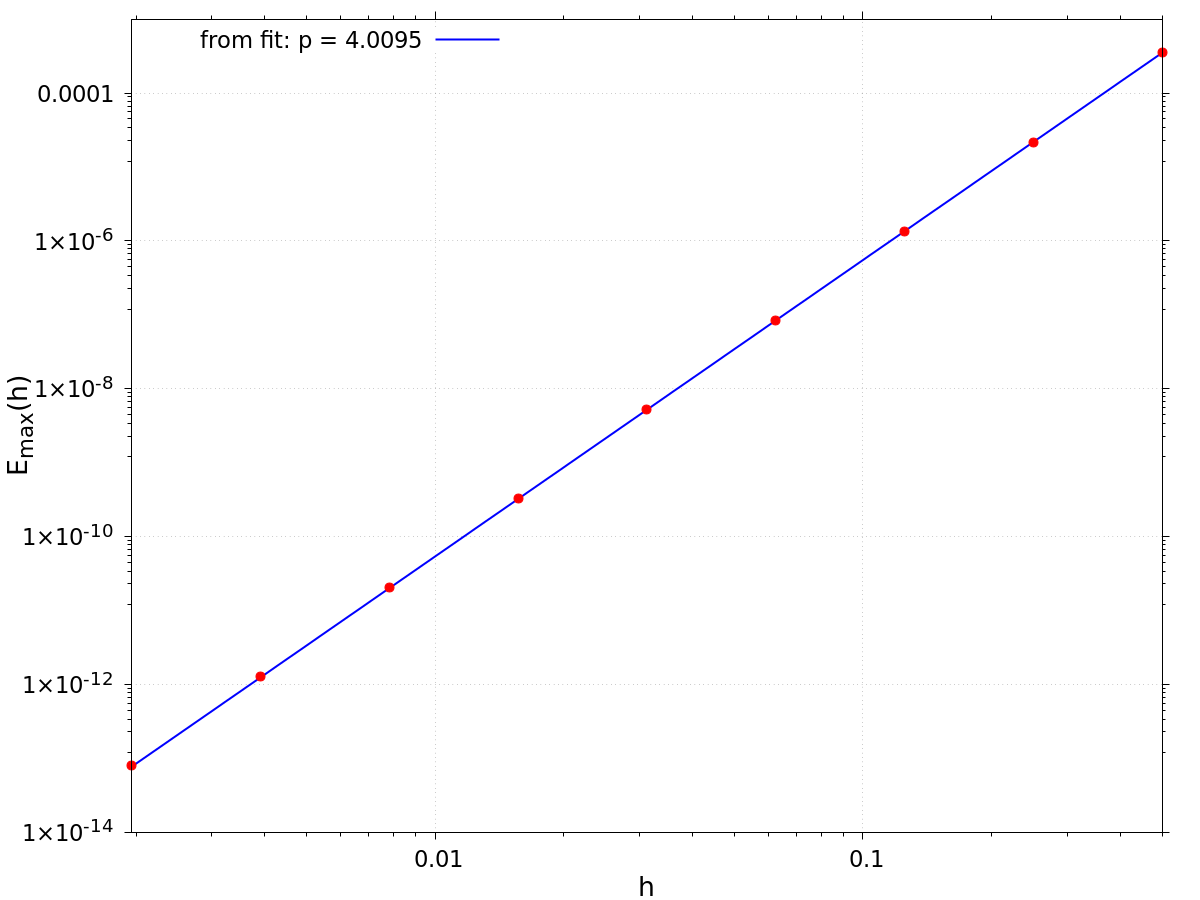
\includegraphics[width=0.5\linewidth]{Immagini/fit_convergenza_RK4.png}
    \caption{fit di $E_{max}(h)$ per la stima di $p$.}
    \label{fig: fit convergenza RK4}
\end{figure}

\subsection{Integrazione dell'equazione di Lane-Emden}
In generale, per poter utilizzare un algoritmo per la soluzione di sistemi di equazioni differenziali ordinarie di secondo ordine, è conveniente riscrivere l'equazione come un sistema di due equazioni differenziali ordinarie del primo ordine. In questo caso, si sono introdotte $Y_0 = \theta(\xi)$ e $Y_1 = \theta'(\xi)$, così da avere il sistema
\begin{equation}
\label{eq: scomposizione sistema del I ordine}
    \begin{cases}
        \dfrac{dY_0}{d\xi} = Y_1 \\[2ex]
        \dfrac{dY_1}{d\xi} = -\dfrac{2}{\xi}Y_1 - \theta(\xi)^n
    \end{cases}.
\end{equation}
Questa forma è implementata nella funzione \texttt{LaneEmdenRHS(double xi, double *Y, double *R)}, dove \texttt{Y[0]} rappresenta $\theta(\xi)$, \texttt{Y[1]} rappresenta $\theta'(\xi)$, mentre \texttt{R[0]} e \texttt{R[1]} sono i membri di destra delle equazioni \eqref{eq: scomposizione sistema del I ordine} rispettivamente. L'indice politropico $n$ viene memorizzato nella variabile globale \texttt{g\_n}, in modo che la funzione \texttt{LaneEmdenRHS} possa essere utilizzata direttamente dall'algoritmo RK4 per valori differenti di $n$.

Una difficoltà nell'integrazione dell'equazione di Lane-Emden è la presenza del termine $2/\xi$, singolare nell'origine. La soluzione regolare viene quindi approssimata nell'intervallo $0 \leq \xi \leq \varepsilon$, con $\varepsilon = 10^{-6}$, mediante lo sviluppo in serie \eqref{eq: sviluppo intorno all'origine} e la sua derivata. Il codice valuta queste espressioni nei punti scelti per il campionamento del tratto iniziale. Raggiunto $\xi = \varepsilon$, i valori ottenuti vengono assegnati a \texttt{Y[0]} e \texttt{Y[1]} e utilizzati come condizioni iniziali per RK4. L'integrazione dell'equazione completa prosegue quindi con passo $\delta\xi = 10^{-3}$, mentre il limite massimo utilizzato per la ricerca della superficie nei singoli casi è $\xi_{max} = 50.0$.

Per evitare problemi numerici quando $\theta$ assume valori negativi, nella funzione \texttt{LaneEmdenRHS} il termine $\theta^n$ viene valutato solamente quando $\theta>0$. Il codice inizializza infatti \texttt{thetan} a zero e assegna
\texttt{pow(theta, g\_n)} soltanto nel caso in cui $\theta$ sia positiva. Questa precauzione è necessaria soprattutto per indici politropici non interi, come $n=3/2$, poiché una potenza frazionaria di un numero negativo non fornirebbe un valore reale. Dal punto di vista fisico, inoltre, per $n<5$ il primo zero di $\theta$ identifica la superficie del sistema, per cui la soluzione di interesse termina in corrispondenza di tale punto. 

A proposito della determinazione del primo zero di $\theta$, ad ogni passo di integrazione vengono confrontati il valore precedente $\theta_{prev}$ e quello corrente $\theta$. Se si verifica la condizione $\theta_{prev}>0$ e $\theta\leq0$, significa che la funzione ha attraversato lo zero durante l'ultimo intervallo di integrazione. Poiché il passo numerico è finito, il valore dello zero non coincide necessariamente con uno dei punti della griglia; per questo motivo il codice non assume semplicemente come superficie l'ultimo punto calcolato, ma effettua un'interpolazione lineare tra i due valori che racchiudono lo zero, ossia con
\begin{equation}
    \xi_s = \xi_{prev}-\theta_{prev}\frac{\xi-\xi_{prev}}{\theta-\theta_{prev}}.
\end{equation}
La stessa interpolazione viene applicata alla derivata per ottenere una stima di $\theta'(\xi_s)$ con
\begin{equation}
    \theta'(\xi_s) = \theta'_{prev} + \left(\theta'-\theta'_{prev}\right)\frac{\xi_s-\xi_{prev}}{\xi-\xi_{prev}}.
\end{equation}
Il valore ottenuto viene memorizzato nella variabile \texttt{g\_thetaPrime\_s}, mentre \texttt{g\_found\_surface} viene posto uguale a $1$ per indicare che la superficie è stata individuata. La funzione \texttt{SolveLaneEmden} restituisce quindi $\xi_s$. Nel caso in cui nessun attraversamento dello zero viene rilevato entro $\xi_{\max}$, la funzione restituisce $-1.0$ e \texttt{g\_found\_surface} rimane uguale a zero.

Per verificare il comportamento della soluzione numerica sono stati considerati gli indici politropici $n = \{0,1,3/2,2,3,4,5\}$. Per ogni valore viene generato un file contenente la coordinata $\xi$, la funzione $\theta(\xi)$ e il termine $\theta(\xi)^n$, proporzionale alla densità adimensionale. I file contengono dapprima i punti calcolati mediante lo sviluppo in serie nell'intervallo $[0,\varepsilon]$, incluso il punto iniziale $(\xi,\theta,\theta^n) = (0,1,1)$, e successivamente quelli ottenuti mediante RK4 per $\xi > \varepsilon$. In questo modo i grafici rappresentano la soluzione a partire dall'origine. Soluzioni e profili di densità sono riportati nelle figure \ref{fig: soluzioni LEE} e \ref{fig: profili densità}, rispettivamente.
\begin{figure}[h]
    \centering
    \begin{minipage}[t]{0.49\linewidth}
        \centering
        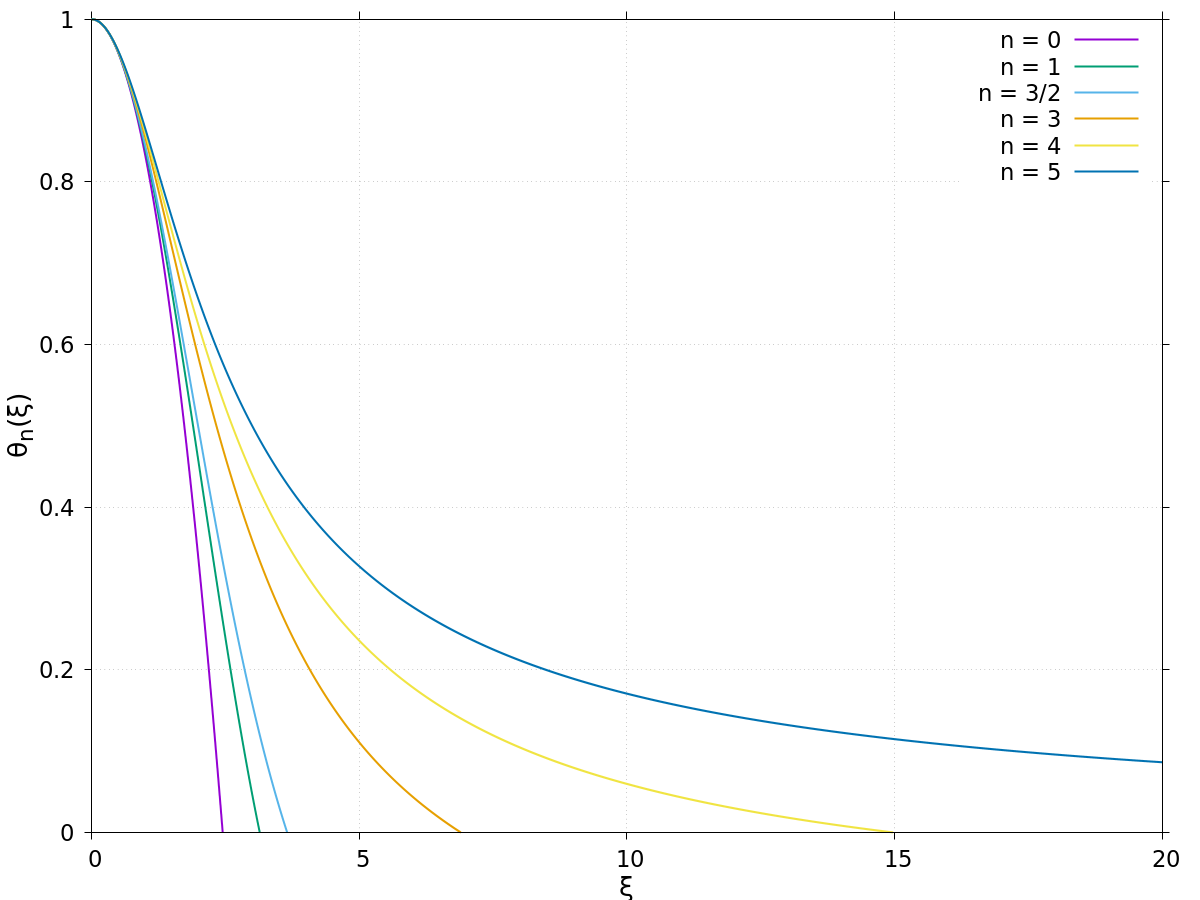
\includegraphics[width=\linewidth]{Immagini/soluzioni_LEE.png}
        \caption{soluzioni dell'equazione di Lane-Emden.}
        \label{fig: soluzioni LEE}
    \end{minipage}
    \hfill
    \begin{minipage}[t]{0.49\linewidth}
        \centering
        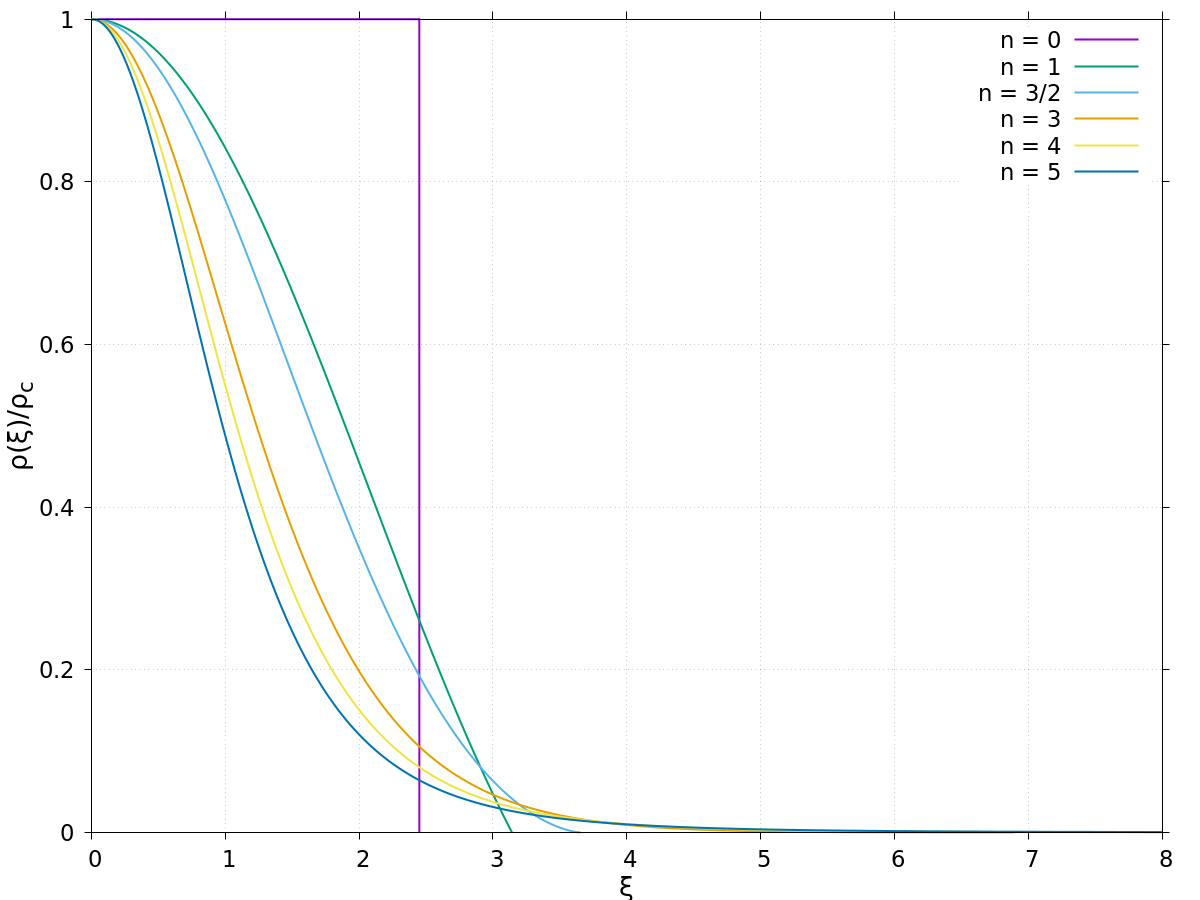
\includegraphics[width=\linewidth]{Immagini/profilo_densità.png}
        \caption{profili di densità.}
        \label{fig: profili densità}
    \end{minipage}
\end{figure}

\subsubsection{Integrazione per \texorpdfstring{$n = 0$}{n = 0} e \texorpdfstring{$n = 1$}{n = 1}}
I casi corrispondenti a $n = 0$, $n = 1$ ed $n = 5$ ammettono soluzioni le analitiche già viste nelle equazioni \eqref{eq: soluzione per n = 0}, \eqref{eq: soluzione per n = 1} e \eqref{eq: soluzione analitica per n = 5} rispettivamente, ma solo nei primi due casi la funzione $\theta(\xi)$ ammette uno zero a $\sqrt{6}$ e $\pi$ rispettivamente. Il terminale per questi due casi restituisce i seguenti valori. 
\begin{verbatim}
    caso n = 0: 
    xi_s = 2.44948989133, (analitico sqrt(6) = 2.44948974278), 
    theta'(xi_s) = -0.816089354022,
    errore massimo = 3.33265299794e-07
    
    caso n = 1: 
    xi_s = 3.14159273049, (analitico pi = 3.14159265359),
    theta'(xi_s) = -0.318309868342,
    errore massimo = 5.55111512313e-15
\end{verbatim}
Per $n = 0$, il massimo errore assoluto della soluzione numerica rispetto a quella analitica risulta dell'ordine di $10^{-7}$, mentre per $n = 1$ dell'ordine di $10^{-15}$, mostrando in entrambi i casi un ottimo accordo tra soluzione numerica e analitica, come mostrato nelle figure \ref{fig: confronto n = 0} e \ref{fig: confronto n = 1} rispettivamente.
\begin{figure}[htbp]
    \centering
    \begin{minipage}[t]{0.49\linewidth}
        \centering
        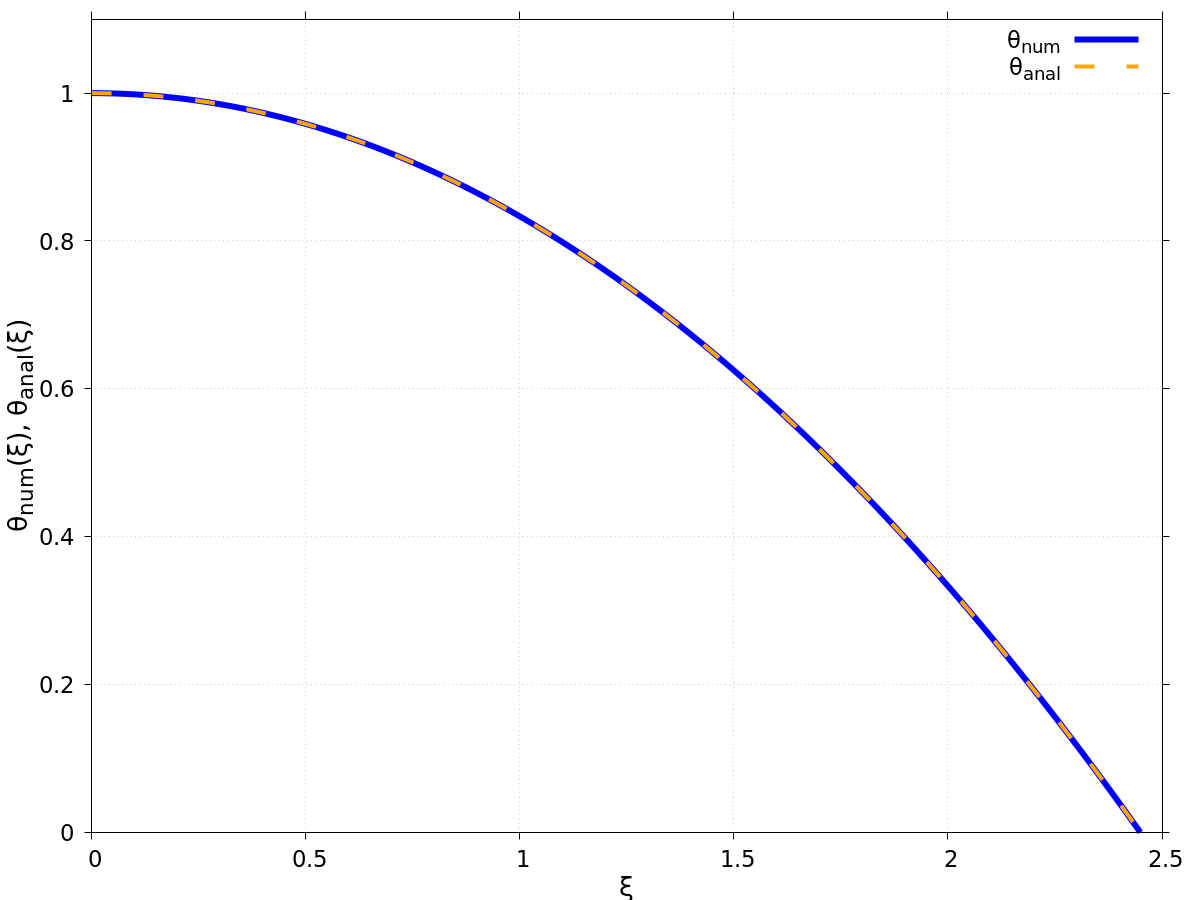
\includegraphics[width=\linewidth]{Immagini/confronto_n0.png}
        \caption{confronto tra soluzione numerica ed analitica per $n = 0$.}
        \label{fig: confronto n = 0}
    \end{minipage}
    \hfill
    \begin{minipage}[t]{0.49\linewidth}
        \centering
        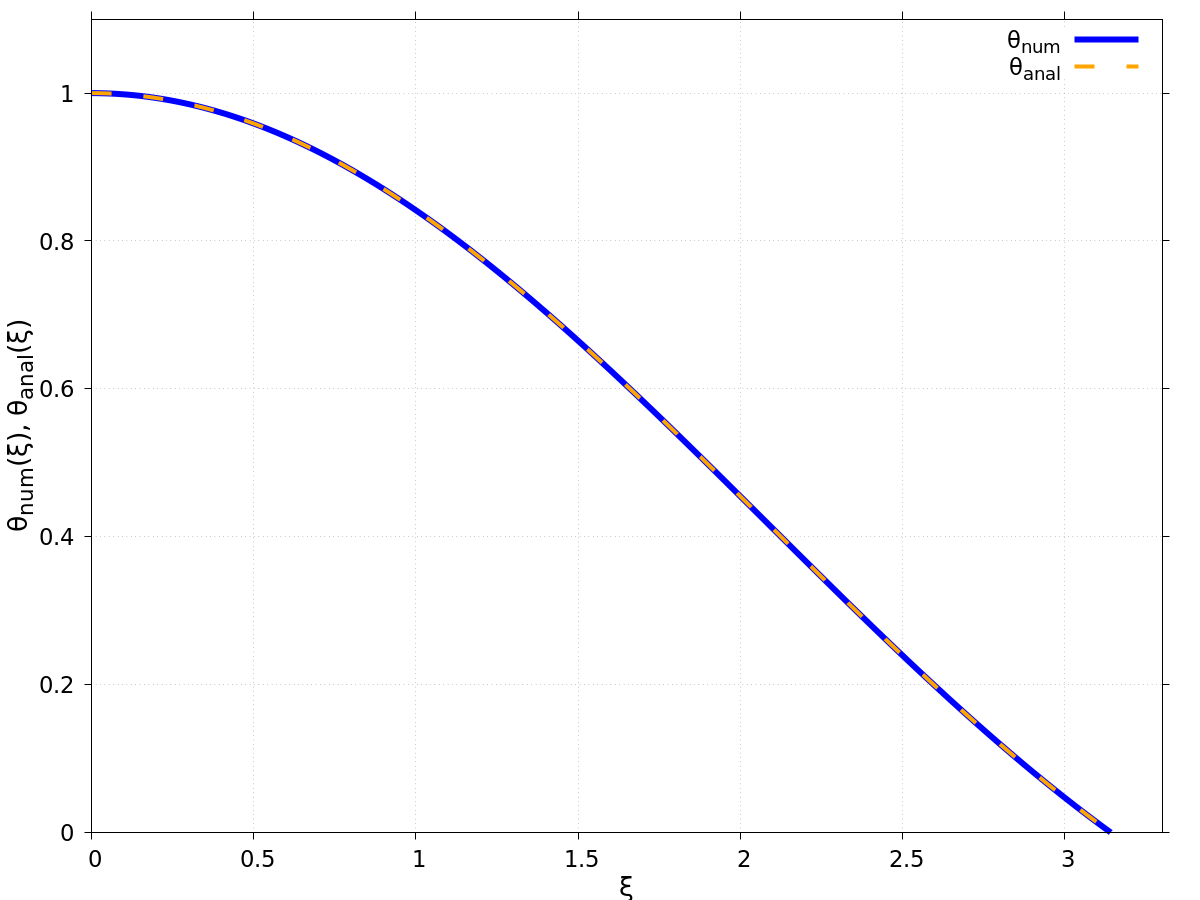
\includegraphics[width=\linewidth]{Immagini/confronto_n1.png}
        \caption{confronto tra soluzione numerica ed analitica per $n = 1$.}
        \label{fig: confronto n = 1}
    \end{minipage}
\end{figure}

\subsubsection{Integrazione per \texorpdfstring{$n = 3/2$}{n = 3/2}, \texorpdfstring{$n = 3$}{n = 3} ed \texorpdfstring{$n = 4$}{n = 4}}
Invece, per $n = 3/2$, $n = 3$ e $n = 4$ non è disponibile una soluzione analitica elementare, e il primo zero viene quindi determinato numericamente. Il terminale restituisce i seguenti valori.
\begin{verbatim}
    caso n = 3/2: 
    xi_s = 3.65375378716, theta'(xi_s) = -0.203301285326

    caso n = 3: 
    xi_s = 6.8968486381, theta'(xi_s) = -0.0424297577197

    caso n = 4: 
    xi_s = 14.9715463654, theta'(xi_s) = -0.00801807881527
\end{verbatim}
Si osserva quindi che, aumentando l'indice politropico, il primo zero della soluzione si sposta progressivamente verso valori maggiori di $\xi$, mentre il valore assoluto di $\theta'(\xi_s)$ diminuisce. La configurazione risulta pertanto sempre più estesa nella coordinata adimensionale all'aumentare di $n$.

\subsubsection{Integrazione per \texorpdfstring{$n = 5$}{n = 5}}
Il caso $n = 5$ è particolarmente significativo perché costituisce il limite tra le configurazioni con raggio finito e quelle che tendono asintoticamente a zero. Infatti, la soluzione analitica \eqref{eq: soluzione analitica per n = 5} rimane positiva per ogni valore finito di $\xi$ e tende asintoticamente a zero per $\xi\rightarrow\infty$. Di conseguenza, la politropa con $n = 5$ non ammette una superficie a raggio finito. Il programma genera il file \texttt{laneemden\_n5\_anal.dat} contenente la soluzione analitica fino a $\xi_{max} = 50$ e, durante l'integrazione, calcola il massimo errore assoluto rispetto alla soluzione numerica. Poiché $\theta_5(\xi)$ non attraversa mai lo zero nell'intervallo considerato, la condizione utilizzata per individuare la superficie non viene soddisfatta e \texttt{g\_found\_surface} rimane uguale a zero. Il massimo errore numerico risulta dell'ordine di $10^{-14}$, mostrando anche in questo caso un ottimo accordo tra integrazione numerica e soluzione analitica, come mostrato in figura \ref{fig: confronto n = 5}.
\begin{figure}[h]
    \centering
    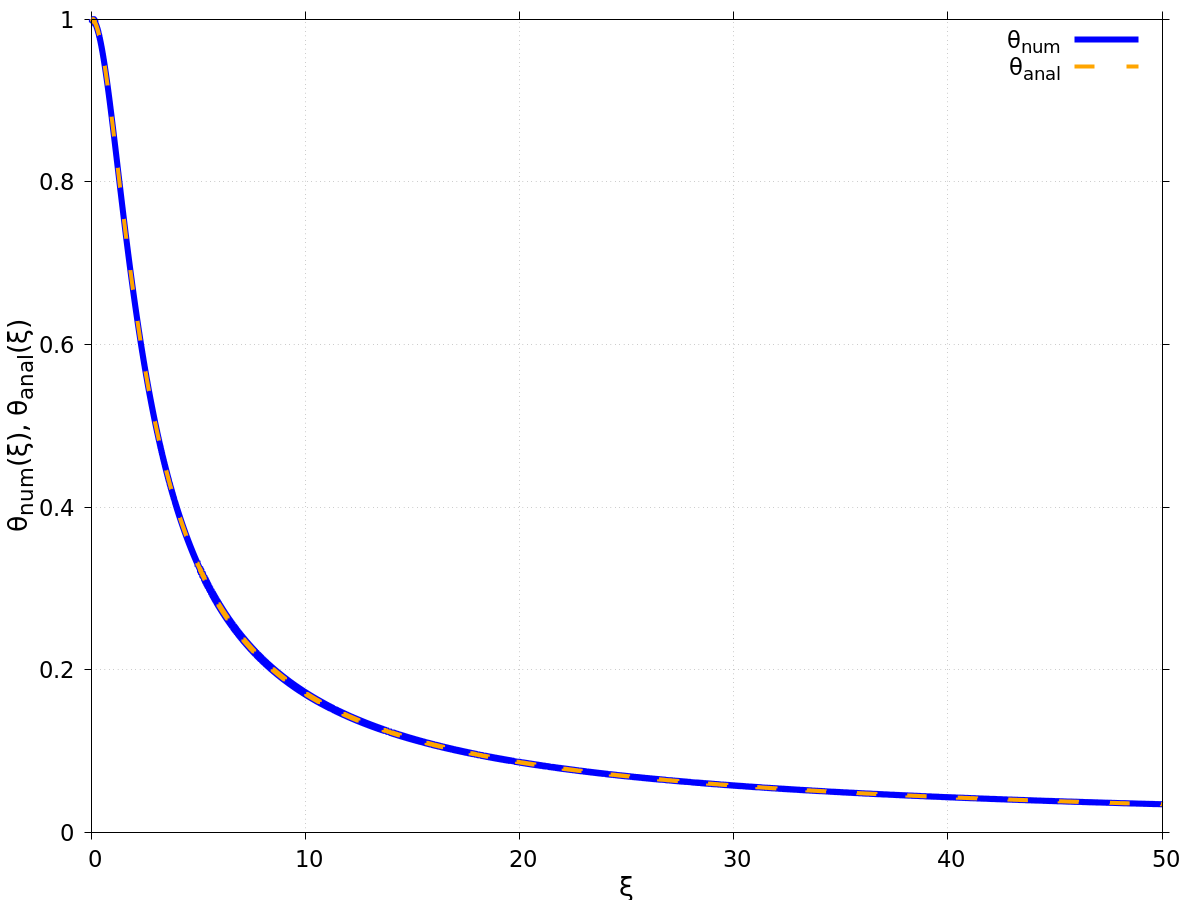
\includegraphics[width=0.49\linewidth]{Immagini/confronto_n5.png}
    \caption{confronto tra soluzione numerica ed analitica per $n = 5$.}
    \label{fig: confronto n = 5}
\end{figure}

\subsubsection{Studio del coefficiente \texorpdfstring{$-\xi_s^2\theta'(\xi_s)$}{-xis2 theta'(xis)}}
Oltre allo studio dei singoli valori di $n$, il programma analizza la dipendenza dall'indice politropico del coefficiente $-\xi_s^2\theta'(\xi_s)$. A questo scopo vengono effettuate successive integrazioni per valori di $n$ compresi tra $0$ e $4.99$. In questa parte del programma viene utilizzato un valore massimo maggiore,
$\xi_{max}^{(coeff)}=1800$, poiché il primo zero della soluzione si sposta rapidamente verso valori elevati di $\xi$ quando $n$ si avvicina a cinque. Per ogni valore di $n$, il programma salva nel file \texttt{laneemden\_mass\_coefficient.dat} il valore di $n$, la posizione della superficie $\xi_s$ e il coefficiente $-\xi_s^2\theta'(\xi_s)$, purché la superficie venga effettivamente individuata. Il raffinamento della griglia vicino a $n = 5$ permette di descrivere con maggiore dettaglio il comportamento della soluzione nella regione in cui $\xi_s$ cresce rapidamente. I risultati sono mostrati nelle figure \ref{fig: zeri soluzioni LEE} e \ref{fig: coefficiente massa}.
\begin{figure}[htbp]
    \centering
    \begin{minipage}[t]{0.49\linewidth}
        \centering
        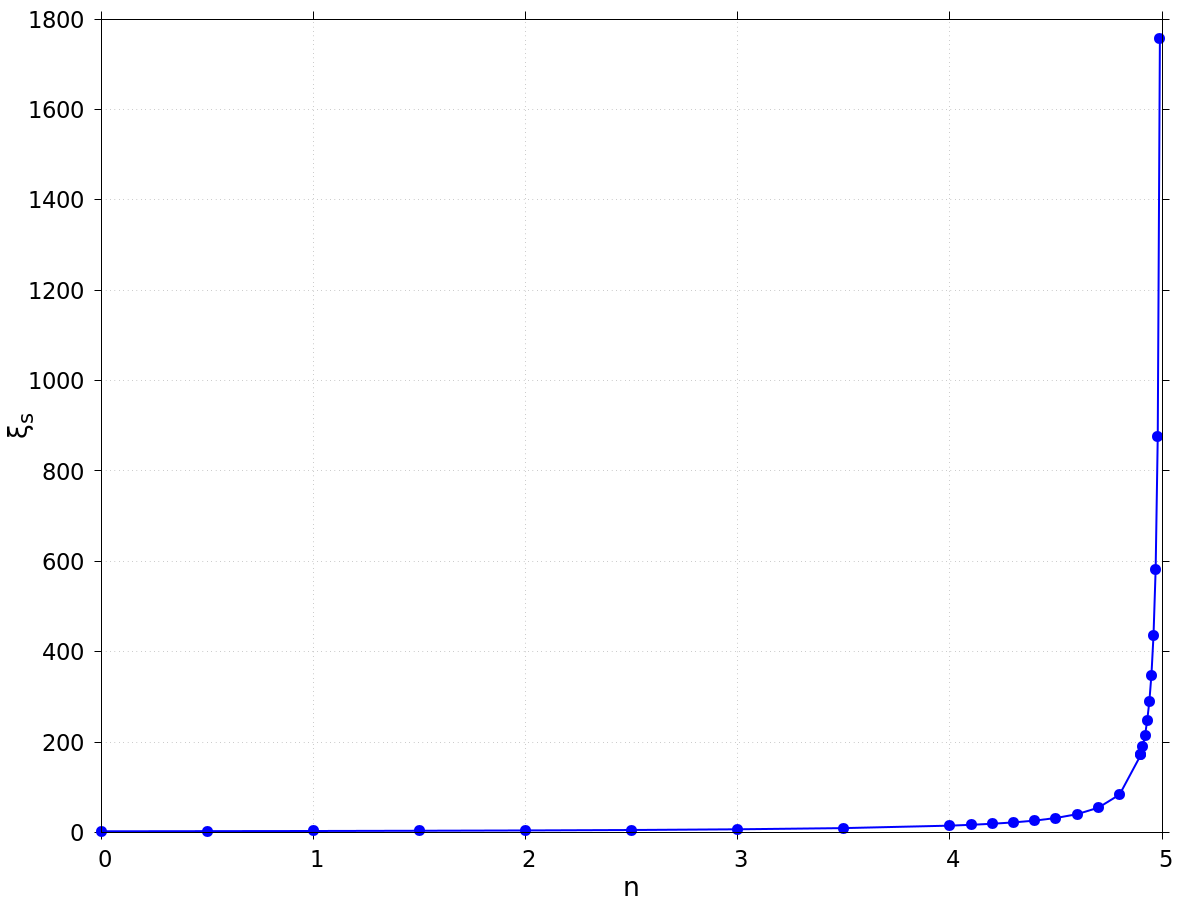
\includegraphics[width=\linewidth]{Immagini/zeri_soluzioni_LEE.png}
        \caption{zeri di $\theta_n(\xi)$ in funzione di $n$.}
        \label{fig: zeri soluzioni LEE}
    \end{minipage}
    \hfill
    \begin{minipage}[t]{0.49\linewidth}
        \centering
        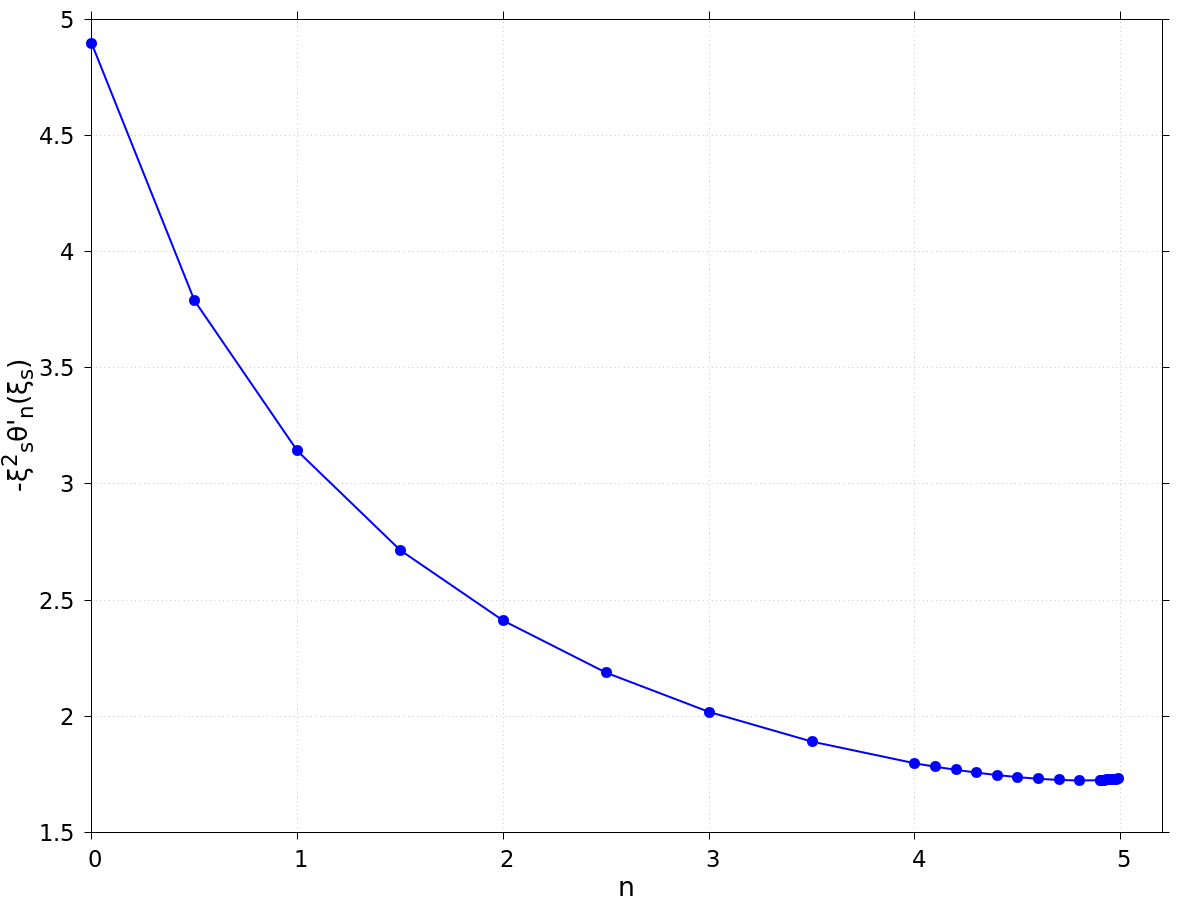
\includegraphics[width=\linewidth]{Immagini/coefficiente_massa_n.png}
        \caption{coefficiente $-\xi_s^2\theta'_n(\xi_s)$ in funzione di $n$.}
        \label{fig: coefficiente massa}
    \end{minipage}
\end{figure}

\subsection{Stima della massa di Chandrasekhar}
Il calcolo della massa limite di Chandrasekhar è stato effettuato considerando il caso con indice $n = 3$, associato al modello per una nana bianca come visto sopra. Per il calcolo servono lo zero della politropa $\theta_3(\xi)$ e il valore del coefficiente adimensionale $\omega \equiv -\xi_s^2\theta_3'(\xi_s)$, il quale compare direttamente nell'espressione della massa di una nana bianca generica \eqref{eq; massa nana bianca generica} e in quella della massa di Chandrasekhar \eqref{eq: massa di Chandrasekhar}, dipendente esclusivamente dall'indice politropico. Si definisce poi la costante\footnote{Considerando un gas di Fermi degenere si ha, nel limite $P_F \gg m_ec$, che 
\begin{equation}
    p = \frac{3^{1/3}\pi^{2/3}}{4}\hbar c n_e^{4/3} = \frac{3^{1/3}\pi^{2/3}}{4}\frac{\hbar c}{(\mu m_p)^{4/3}}\rho^{4/3},
\end{equation}
dove si è scritta la densità di elettroni tramite la relazione $\rho = \mu m_p n_e$. Confrontando quest'ultima equazione con l'equazione di stato politropica $p = K\rho^{4/3}$ per $n = 3$ si ottiene proprio la costante $K$ in questione. Per maggiori dettagli si veda \cite[pg.~2,pg.~5]{chavanis2007}.} $K$ presente nell'equazione di stato politropica \eqref{eq: equazione di stato politropica} legata al gas di elettroni completamente degenere e relativistico come
\begin{equation}
    K = \frac{3^{1/3}\pi^{2/3}}{4}\frac{\hbar c}{(2m_p)^{4/3}}.
\end{equation}
La massa viene quindi calcolata mediante la funzione \texttt{PolytropeMass()}, nella quale viene calcolato
\begin{equation}
    \alpha = \sqrt{\frac{(n + 1)}{4\pi G}K}\rho_c^{(1 - n)/2n},
\end{equation}
con il quale di determina la massa di Chandrasekhar tramite
\begin{equation}
\label{eq: massa di Chandrasekhar in funzione di alpha}
    M_C = 4\pi \alpha^3\rho_c \omega.
\end{equation}
La formula per $M_C$ in questa forma deriva direttamente dalla definizione
\begin{equation}
    M(r) = 4\pi\int_0^r\rho(r')r'^{\,2}\,dr'
\end{equation}
che, sostituendo $r = \alpha\xi$ e $\rho = \rho_c\theta^n$, diventa
\begin{equation}
    M(\xi) = 4\pi \alpha^3\rho_c\int_0^\xi \xi'^{\,2}\theta(\xi')^n\,d\xi'.
\end{equation}
Usando ora l'equazione \eqref{eq: equazione di Lane-Emden} si può derivare l'integrale da cui dipende $M(\xi)$, 
\begin{equation}
    \omega \equiv -[\xi_s^2\theta_3'(\xi_s)] = \int_0^{\xi_s}\xi^2\theta_3(\xi)^n\,d\xi,
\end{equation}
trovando quindi la relazione in questione. Inoltre, la relazione \eqref{eq: massa di Chandrasekhar in funzione di alpha} è equivalente a quella in equazione \eqref{eq: massa di Chandrasekhar}, questo si può vedere sostituendo $\alpha^3\rho_c$ e la costante $K$ con le espressioni note\supcite[pg.~3]{chavanis2007}.

Ad ogni modo, il calcolo viene effettuato per valori diversi di $\rho_c$ in modo da verificare numericamente anche l'indipendenza di $M_C$ da tale quantità. Infatti, sostituendo $n = 3$ nell'esponente della dipendenza di $a$ da $\rho_c$, si ottiene $a \propto \rho_c^{-1/3}$ e quindi $a^3\rho_c\propto\rho_c^{-1}\rho_c = 1$, da cui segue l'eliminazione completa della dipendenza dalla densità centrale. Per evidenziare quantitativamente questa proprietà, il programma calcola anche le differenze percentuali tra le masse ottenute ai diversi valori di $\rho_c$, verificando che esse risultano estremamente piccole e compatibili con i soli errori numerici dell'integrazione. Oltre alla massa, viene calcolato anche il raggio della configurazione utilizzando la funzione \texttt{PolytropeRadius()}, che implementa la relazione $R = \alpha\xi_s$. Poiché nel caso $n = 3$ risulta $a \propto \rho_c^{-1/3}$, il raggio diminuisce all'aumentare della densità centrale, mantenendo la massa costante. Il terminale restituisce i seguenti valori.
\begin{verbatim}
    rho_c [kg/m^3]  M [M_sun]        R [R_sun]
    1.000000e+08    1.435289855520   0.103114793357
    1.000000e+09    1.435289855520   0.047861647343
    1.000000e+10    1.435289855520   0.022215408786
    1.000000e+11    1.435289855520   0.010311479336
    1.000000e+12    1.435289855520   0.004786164734
\end{verbatim}
La massima variazione relativa della massa nell'intervallo di densità considerato risulta pari a $4.64\times10^{-14}\%$, confermando che la massa è indipendente da $\rho_c$ entro la precisione numerica del calcolo. Il raggio diminuisce invece da circa $0.1031\,R_\odot$ a $0.004786\,R_\odot$, coerentemente con la dipendenza $R \propto \rho_c^{-1/3}$.

\section{Conclusioni}
In conclusione, in questo progetto si è studiata numericamente l'equazione di Lane-Emden in funzione dell'indice politropico utilizzando il metodo RK4. Per trattare la singolarità presente nell'origine, la soluzione è stata approssimata mediante lo sviluppo in serie nell'intervallo $0 \leq \xi \leq \varepsilon$, con $\varepsilon = 10^{-6}$, e successivamente calcolata mediante RK4 utilizzando come dati iniziali i valori della funzione e della sua derivata ottenuti a $\xi = \varepsilon$. La posizione della superficie delle configurazioni con $n < 5$ è stata quindi determinata individuando il primo zero $\xi_s$ di $\theta(\xi)$ e applicando un'interpolazione lineare per stimare con maggiore precisione sia $\xi_s$ sia $\theta'(\xi_s)$.

I casi $n = 0$, $n = 1$ e $n = 5$, per i quali sono disponibili soluzioni analitiche, hanno permesso di verificare l'affidabilità dell'integrazione numerica. Per $n = 0$ e $n = 1$ sono stati ottenuti valori del primo zero rispettivamente pari a $\xi_s \simeq 2.44949$ e $\xi_s \simeq 3.14159$, in ottimo accordo con i valori teorici $\sqrt{6}$ e $\pi$. Nel caso $n = 5$, invece, la soluzione rimane positiva e tende asintoticamente a zero, confermando l'assenza di una superficie a raggio finito. Anche per i casi privi di soluzione analitica elementare, $n = 3/2$, $n = 3$ e $n = 4$, il metodo ha permesso di determinare numericamente la struttura delle politrope e di osservare che il primo zero $\xi_s$ aumenta progressivamente con l'indice politropico.

L'accuratezza dell'algoritmo è stata ulteriormente verificata attraverso uno studio di convergenza nel caso $n = 1$. Dimezzando progressivamente il passo di integrazione, l'errore massimo diminuisce approssimativamente di un fattore $16$, mentre l'ordine di convergenza osservato risulta molto vicino a $p = 4$, in accordo con il comportamento teorico atteso per il metodo RK4. Inoltre, il fit dei dati tramite $E_{max}(h) = ah^p$ restituisce $p = 4.0095$. Sia l'ordine locale sia quello ottenuto dal fit risultano quindi in accordo con il comportamento teorico atteso. Questi risultati confermano la correttezza dell'implementazione e giustifica l'utilizzo del passo $\delta\xi = 10^{-3}$ nelle integrazioni finali.

Particolare attenzione è stata infine dedicata al caso $n = 3$, corrispondente al limite relativistico di una nana bianca sostenuta dalla pressione di degenerazione elettronica. La soluzione numerica fornisce $\xi_s \simeq 6.89685$ e il coefficiente
\begin{equation}
    \omega \equiv -\xi_s^2\theta_3'(\xi_s)\simeq2.01824,
\end{equation}
in accordo con il valore teorico associato alla soluzione di Lane-Emden con indice $n = 3$. Utilizzando questo risultato nell'espressione della massa politropica è stata ottenuta una massa limite
\begin{equation}
    M_C \simeq 1.4353\, M_\odot,
\end{equation}
compatibile con il valore atteso della massa di Chandrasekhar di $1.44\, M_\odot$. Il calcolo è stato ripetuto per densità centrali pari a $10^8$, $10^9$, $10^{10}$, $10^{11}$ e $10^{12}$ $\mathrm{kg\,m^{-3}}$, verificando numericamente l'indipendenza di $M_C$ da $\rho_c$. Al contrario, si è osservato che il raggio diminuisce all'aumentare di $\rho_c$, passando da circa $0.103\, R_\odot$ a $0.00479\, R_\odot$ nell'intervallo di densità considerato, coerentemente con la dipendenza $R \propto \rho_c^{-1/3}$.

\newpage
\appendix

\newgeometry{left=2.36cm,right=2.36cm,top=2.5cm,bottom=2.5cm}

\section{Codice}
\label{app: appendice}

\subsection{Header}
\lstinputlisting[language=C++]{Codice/LaneEmdenLibrary.hpp}

\subsection{Implementazione}
\lstinputlisting[language=C++]{Codice/LaneEmdenLibrary.cpp}

\subsection{Main}
\lstinputlisting[language=C++]{Codice/LaneEmden.cpp}

\subsection{Gnuplot}
\lstinputlisting{Codice/LaneEmden.gp}

\restoregeometry

\newpage
\printbibliography[heading=bibintoc, title={Bibliografia}]

\newpage
\tableofcontents

\end{document}

